\section{Computational Complexity of Real Functions}
\label{section: preliminaries}

This section reviews the complexity notions 
in Computable Analysis~%
\cite{ko1991complexity,weihrauch00:_comput_analy}. 
We start by fixing an encoding of real numbers 
by string functions.

\begin{definition}
 A function $\phi \colon \{0\} ^* \to \{0, 1\}^*$ is a \emph{name} of a real number $x$ 
 if for all $n \in \N$,
  $\phi(0^n)$ is the binary representation of $\lfloor x \cdot 2^n \rfloor$ or
  $\lceil x \cdot 2^n \rceil$,
 where $\lfloor \cdot \rfloor$ and $\lceil \cdot \rceil$ mean
 rounding down and up to the nearest integer.
 \end{definition}

In effect, a name of a real number $x$ receives $0 ^n$ and 
returns an approximation of $x$ with precision $2 ^{-n}$.

We use \emph{oracle Turing machines} (henceforth just \emph{machines})
to work on these names (Fig.~\ref{fig:model-of-function}).
Let $M$ be a machine and $\phi$ be a function from strings to strings. 
We write $M ^\phi (0 ^n)$ for the output string 
when $M$ is given
$\phi$ as oracle and string $0^n$ as input.
Thus we also regard $M^\phi$ as a function from strings to strings.

\begin{figure}
 \begin{center}
  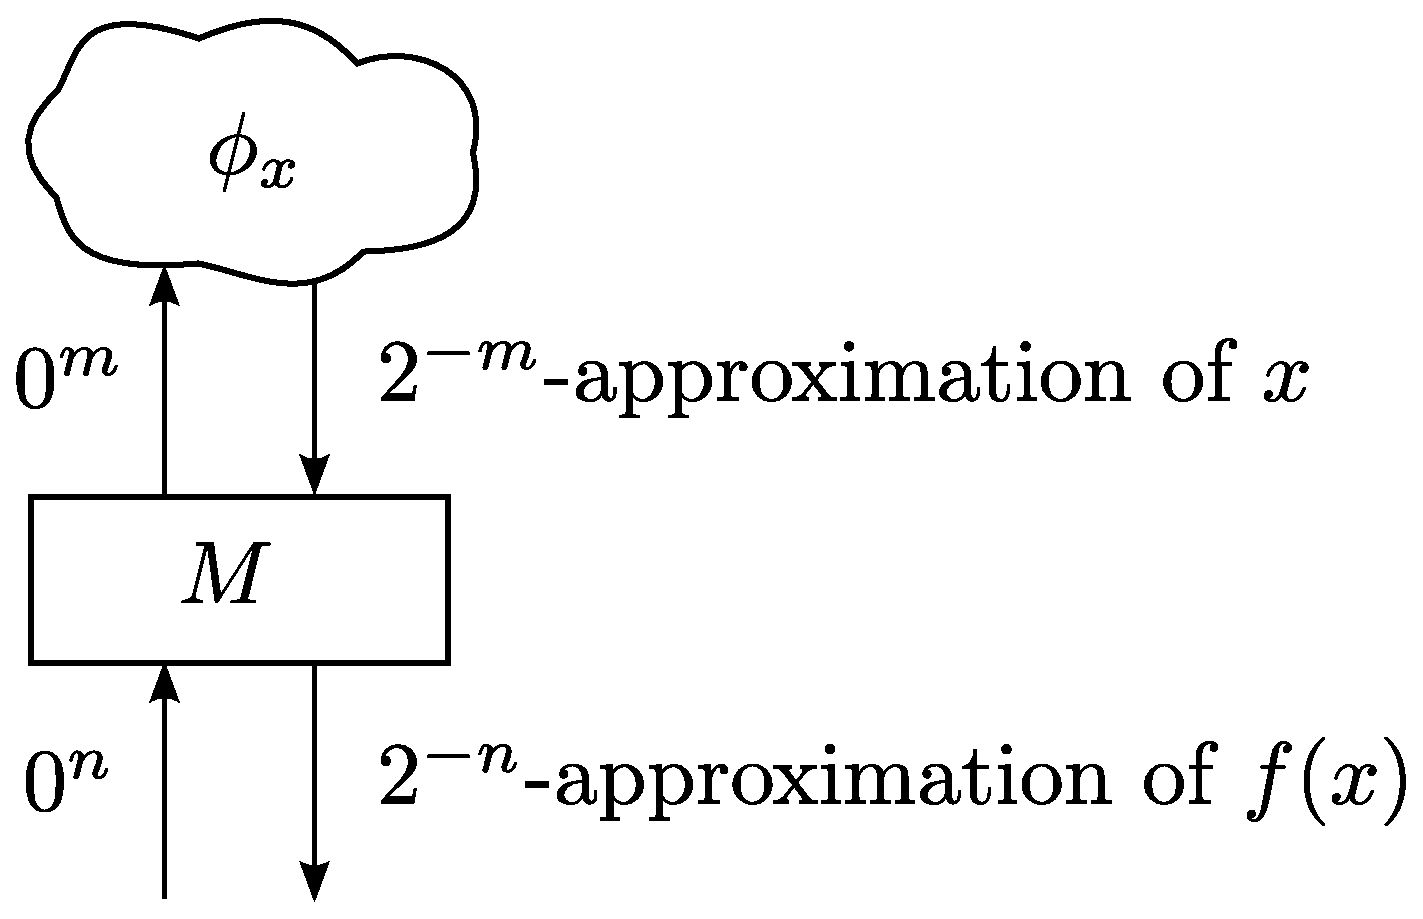
\includegraphics[height=0.17\textheight]{image/model-of-function.eps}
 \end{center}
 \caption{A machine $M$ computing a real function $f$}
 \label{fig:model-of-function}
\end{figure}

\begin{definition}
Let $A$ be a bounded closed interval of\/ $\R$.
A machine $M$ \emph{computes} a real function $f \colon A \to \R$ 
if for any $x \in A$ and any name $\phi_x$ of it,
$M^{\phi_x}$ is a name of $f(x)$.
\end{definition}

Computation of a function $f \colon A \to \R$ on
a two-dimensional bounded closed region $A \subseteq \R ^2$ 
is defined in a similar way using machines with two oracles.
A real function is (\emph{polynomial-time}) \emph{computable} if there exists some machine that computes it (in polynomial time).
Polynomial-time computability of a real function $f$ means that
for any $n \in \N$, 
an approximation of $f(x)$ with error bound $2^{-n}$
is computable in time polynomial in $n$ 
independent of the real number $x$.

By the time the machine outputs the approximation of $f (x)$ of precision~$2 ^{-n}$, 
it knows $x$ only with some precision $2 ^{-m}$.
This implies that all computable real functions are continuous.
If the machine runs in polynomial time,
this $m$ is bounded polynomially in $n$.
This implies \eqref{eq:modulus} in the following lemma, 
which characterizes polynomial-time real functions
by the usual polynomial-time computability of string functions 
without using oracle machines. 

\begin{lemma}
 \label{lem:type1representation}
 A real function is polynomial-time computable if and only if
 there exist a polynomial-time computable function 
 $\phi \colon (\Q \cap [0, 1]) \times \{0\} ^* \to \Q$ and 
 polynomial $p \colon \N \to \N$ such that
 for all $d \in \Q \cap [0,1]$ and $n \in \N$,
 \begin{equation}
  |\phi(d, 0^n) - f(d)| \le 2^{-n},
 \end{equation}
 and for all $x, y \in [0, 1]$, $n \in \N$,
 \begin{equation} 
  |x-y| \le 2^{-p(n)} \Rightarrow |f(x) - f(y)| \le 2^{-n},
   \label{eq:modulus}
 \end{equation}
where each rational number is written
as a fraction whose numerator and denominator
are integers in binary.
\end{lemma}

To talk about hardness, we define reduction. 
A language $L \subseteq \{0, 1\} ^*$ is identified with the function
$L \colon \{0, 1\} ^* \to \{0, 1\}$ such that $L (u) = 1$ when $u \in L$.

\begin{definition} \label{definition: reduction}
 A language $L$ \emph{reduces} to a function $f \colon [0, 1] \to \R$
 if there exists a polynomial-time function $S$ and a polynomial-time oracle Turing machine $M$ (Fig.~\ref{fig:reduction})
 such that for any string $u$, 
  \begin{enumerate}
   \item $S(u, \cdot)$ is a name of a real number $x_u$, and 
   \item $M^\phi(u)$ accepts if and only if $u \in L$ for any name $\phi$ of $f(x_u)$.
  \end{enumerate}
\end{definition}
This reduction may look stronger (and hence the reducibility weaker) than
the one in Kawamura~\cite{kawamura2010lipschitz} 
in that $M$ can make multiple queries adaptively, 
but this makes no difference, 
because the lengths of these queries 
are bounded by a polynomial in $\lvert u \rvert$, 
and the longest query gets all the information that any shorter query gets. 

For a complexity class~$C$, a function $f$ is \emph{$C$-hard}
if all languages in $C$ reduce to $f$.

 \begin{figure}
  \begin{center}
  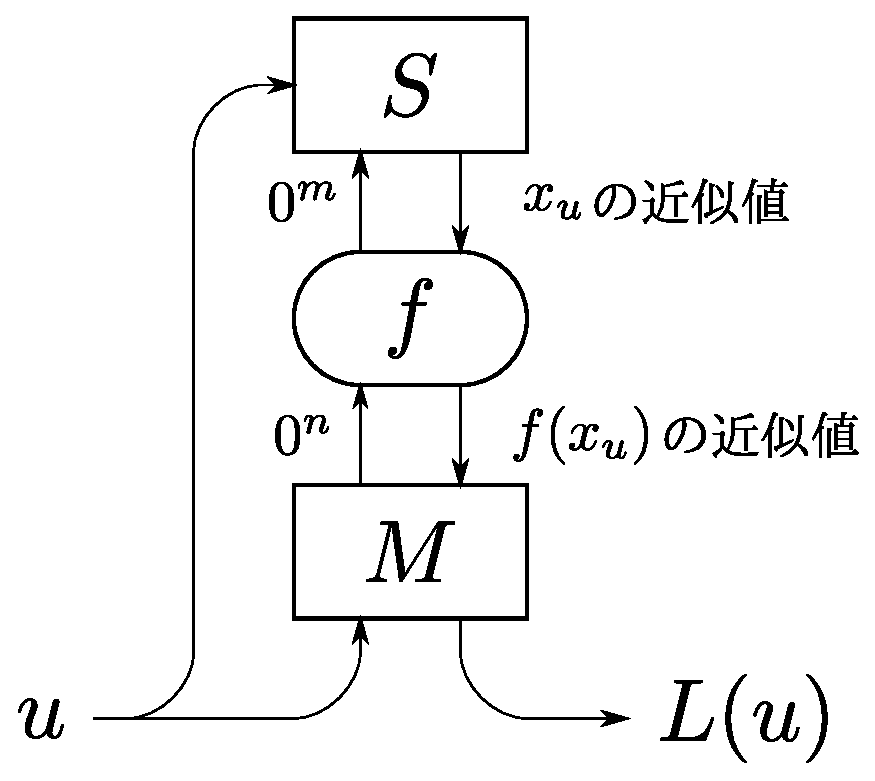
\includegraphics[scale=0.25]{image/reduction.eps}
  \caption{Reduction from a language $L$ to a function $f \colon [0,1] \to \R$}
  \label{fig:reduction}
  \end{center}
 \end{figure}

